\newpage
\section{Approach}
The role mining problems (see section \ref{sec:roleMiningProblems}) have been approached with different problem formulations, techniques and algorithms. In this thesis the approach of solving role mining with an evolutionary algorithms is investigated.\\
Evolutionary algorithms seem to be a promising approach for role mining for several reasons. Role mining is following several objectives, e.g. minimizing the number of roles and minimizing the number of confidentiality and availability violations, which can be in conflict with each other. With multiobjective evolutionary algorithms pareto-optimal solutions, a set of optimal trade-offs solutions, can be found in a single run instead of several runs, which is necessary for some of the conventional stochastic processes, like simulated annealing and tabu search\cite{abraham2005evolutionary}. Previous research in the role mining field are using scalarisation, where several objectives are weighted and summarized in one single objective, like the weighted structural complexity (WSC) in Molloy et al.\cite{Molloy} or the fitness function for the basic RMP in Saenko et al.\cite{saenko2012design}. The trade-offs between the objectives are not apparent in these approaches. Furthermore the task of role engineering is an on-going process. After an initial role model is created, the user-permission relation can change over time and therefore the roles in the role model can become suboptimal. Evolutionary algorithms can adapt solutions to changing circumstances\cite{Fogel:1997}. A current role model state can be used as starting population and the evolutionary algorithm will optimize towards the formulated objective in the fitness functions. At last role engineering is still a process, which requires human interaction. The role mining results are evaluated by humans and modified to an extend that it is accepted by the business. Interactive evolutionary computation (IEC)\cite{949485} could include human feedback to the algorithm to navigate the evolutionary algorithm to an optimal result. In IEC the fitness function is replaced by an human user.\\
Since there has not been a lot of research done up till now (see chapter \ref{sec:relatedWork} for related work), the research in this thesis starts with a basic set up of the domain-specific problem as evolutionary computation problem. The evolutionary algorithm, the representation of an individual, variation operators, selection mechanisms and fitness functions used in this approach are described in the following sections. For handling constraints for an RBAC$_2$ role model, a penalty function and intelligent variation operators are introduced. Furthermore the multiobjective evolutionary algorithm used in this approach is described with its challenges and improvements. In order to come to an human digestible representation of individuals for human feedback in an IEC approach, an alternative approach with a different representation and a Co-Evolution technique is presented.

    \subsection{Overview of the Evolutionary Algorithm}
    The evolutionary algorithm for single objectives used in this thesis is based on the pseudo-code in Algorithm \ref{alg:EA}. The algorithm starts with the initial generation and evaluation of the parent population $P_p$. Then, for each generation, individuals from $P_p$ are selected and cloned as offspring population $P_o$. A loop over neighboring individuals in $P_o$ is mating individuals $\mathbf{x}_i$ and $\mathbf{x}_{i+1}$ by crossover probability $CXPB$. The resulting children $\mathbf{y}_i$ and $\mathbf{y}_{i+1}$ replace their respective parents in $P_o$. In a second loop over all individuals in $P_o$ the individuals get mutated by mutation probability $MUTPB$. The resulting mutation is replacing the original individual. The resulting individuals in $P_o$ can be generated from crossover only, mutation only, crossover and mutation, and reproduction according to the given probabilities $CXPB$ and $MUTPB$. The offspring population $P_o$ is then getting the parent population $P_p$ for the next generation, after each individual got evaluated.\\
    In the following sections, the components within the algorithm are discussed more in detail.
    
    \begin{algorithm}
        \caption{Evolutionary algorithm for single objectives}
        \label{alg:EA}
        \begin{algorithmic}[1]
            \Procedure{eaSingle}{$popSize$, $NGEN$, $CXPB$, $MUTPB$}
                \State $P_p$ = generatePopulation($popSize$)
                \State evaluateIndividuals($P_p$)
                \State $solutionFound$ = False
                \State $generation$ = 1
                \While{not $solutionFound$ AND $generation <= NGEN$}
                    \State $P_p$ = select($population$, k=length($P_p$))
                    \State $P_o$ = clonePopulation($P_p$)
                    \State $i$ = 0
                    \While{ $i < length(P_o)-1$}
                        \State $P_o$[$i$],$P_o$[$i$+1] = crossover($P_o$[$i$],$P_o$[$i$+1],$CXPB$)
                        \State $i$ += 2
                    \EndWhile
                    \State $i$ = 0
                    \While{ $i < length(P_o)$}
                        \State $P_o$[$i$] = mutation($P_o$[$i$],$MUTPB$)
                        \State $i$ += 1
                    \EndWhile
                    \State $P_p$ = $P_o$
                    \State evaluateIndividuals($P_p$)
                    \State $generation$ += 1
                \EndWhile
                \State \Return $result$
            \EndProcedure
        \end{algorithmic}
    \end{algorithm}

    \subsection{Representation of a role model as individual}
    The representation of individuals in an EA is crucial for the success of the EA and influences the variation operators. Finding a good representation of role models as individuals for a Role Mining EA is a challenging task, since the number of roles for a role model is not predefined. In the following one bit-string and two complex representations are introduced and evaluated. The complex representations were proposed by Saenko et al.\cite{saenko2012design}.
        \subsubsection{Representation as Bit-string}
        The representation of individuals as bit-string is one of the simplest and is often mistakenly used in genetic algorithms\cite{Eiben}. A suggestion for a bit-string representation for a role model is derived from a combined user-role- (UA) and role-permission-matrix (PA). Figure \ref{fig:representation1} shows an example of a combined UA- and PA-Matrix and an according bit-string representation.
        \begin{figure}
            \centering
            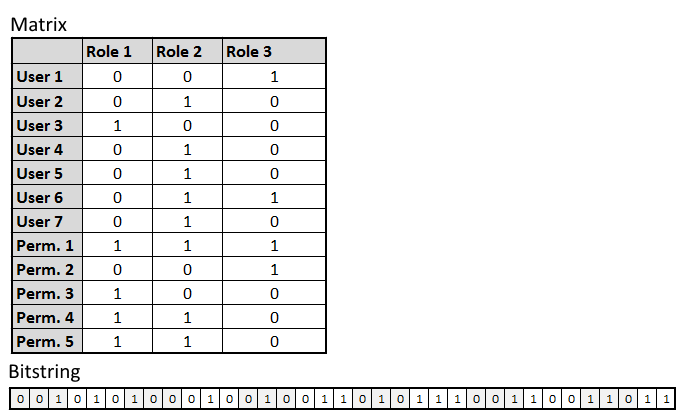
\includegraphics[scale=0.75]{./Figures/Representation1.png}
            \rule{20em}{0.5pt}
            \caption{\textit{Example of a combined UR- and RP-Matrix with its bit-string representation}}
            \label{fig:representation1}
        \end{figure}
        The motivation of this initial idea is that the mutation operator can be easily executed by just flipping a bit within the bit-string. The mutation is therefore adding or removing a user or permission from a role. For the decoding two leading 8-bit integers can represent the number of users and permission. However, the problem with this representation is that the number of roles needs to be pre-defined, such that the bit-string can be decoded again. Alternatively another leading 8-bit integer can represent the number of roles in the role model. But varying the number of roles demands adding or removing bits in the bit-string for each user-role- and role-permission relation. Furthermore the information that a user or a permission is not part of a role seems to unnecessarily lengthens the bit-string, which can consume a lot of space for high-dimensional UA- and PA-Matrices.
        \subsubsection{Representations as Complex Objects}
        In Saenko et al.\cite{saenko2012design} two different representations are introduced, which are briefly described in chapter \ref{sec:relatedWork}. With the first representation the authors suggest a multi-chromosomal representation where the number of roles becomes part of the search. An example can be seen in figure \ref{fig:representation2}. A drawback of this representation are unnecessary genes (roles) like the unneccessary information in the bit-string representation. Another disadvantage of the representation are complex crossover operations\cite{saenko2012design}.
        \begin{figure}
            \centering
            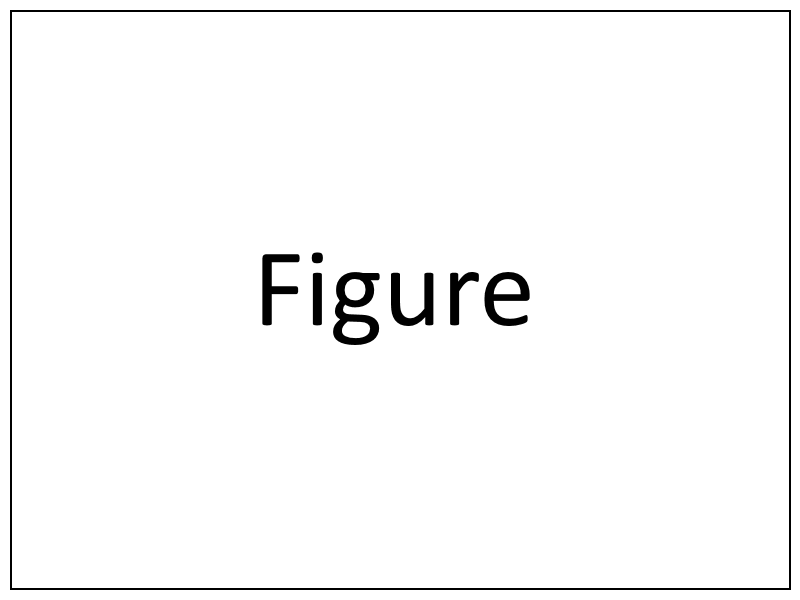
\includegraphics[scale=0.4]{./Figures/dummy.png}
            \rule{20em}{0.5pt}
            \caption{\textit{Description}}
            \label{fig:representation2}
        \end{figure}
        The second improved representation eliminates these drawbacks by having one chromosome for an individual, where no unnecessary genes occur. The chromosome consists of a list of roles, which contain a user-set and a permission-set (see figure \ref{fig:representation3}).\\
        \begin{figure}
            \centering
            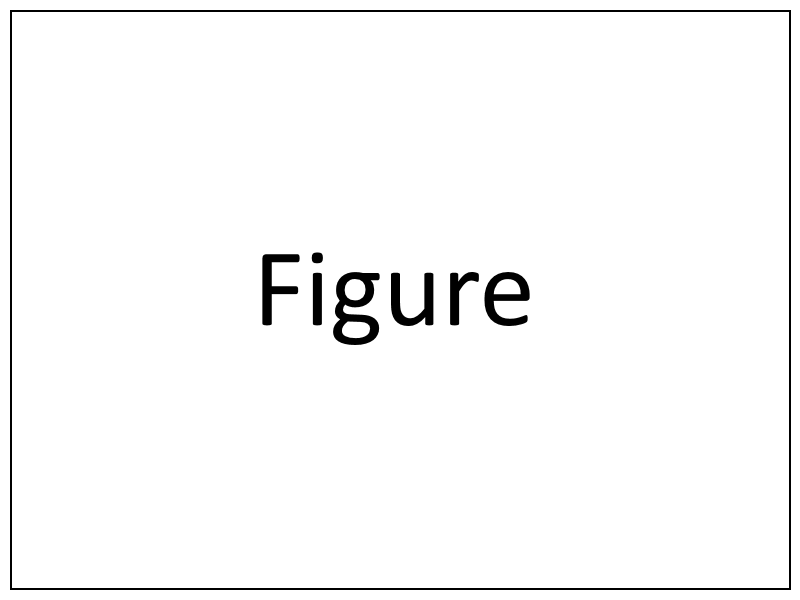
\includegraphics[scale=0.4]{./Figures/dummy.png}
            \rule{20em}{0.5pt}
            \caption{\textit{Description}}
            \label{fig:representation3}
        \end{figure}
        Due to the advantages of the improved representation of Saenko et al.\cite{saenko2012design}, their suggested representation is used for the research in this thesis.
    
    \subsection{Variation Operators on role model representation}
    \hl{SECTION UNDER CONSTRUCTION}\\
    Dependent on the choice of the representation of individuals in the previous section, according mutation and crossover methods are created. The choice of variation operators and how often they are executed influences how much of the search space is discovered during the evolution. Since the improved representation of Saenko et al.\cite{saenko2012design} has been selected for this thesis, the following variation operators are suited for this representation.
        \subsubsection{Mutation methods}
        Since no further instructions for the mutation are given in Saenko et al.\cite{saenko2012design}, the mutation operations have been chosen intuitively. For the mutation six different mutation types are implemented, which are executed in the following order depending on their probability.
        \begin{itemize}
            \setlength{\itemsep}{1pt}
            \item Add a new role
            \item Add a user to a role
            \item Add a permission to a role
            \item Remove a role
            \item Remove a user from a role
            \item Remove a permission from a role
        \end{itemize}
        Examples can be seen in Figure \ref{fig:mutationOperations}. If an individual gets mutated is determined by a fixed probability. In addition fixed probabilities for each mutation method is dictating how the individual gets mutated. The probabilities allow to influence how often a certain mutation should be executed and can therefore influence how much new solutions are discovered and how likely good solutions are lost. The mutation operations are implemented in such a way that it is ensured that all users and permissions are assigned to at least one role. This prevents that incomplete role models can occur.
        \begin{figure}
            \centering
            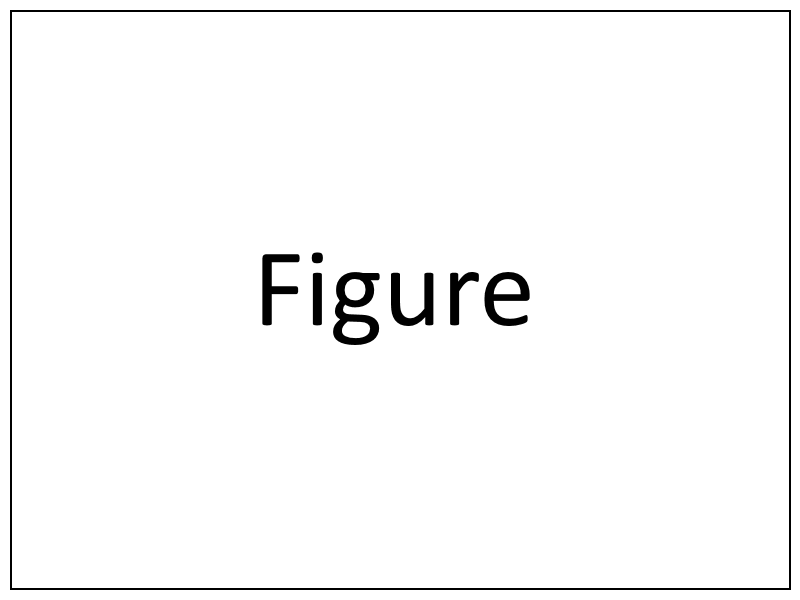
\includegraphics[scale=0.4]{./Figures/dummy.png}
            \rule{20em}{0.5pt}
            \caption{Examples for the six different mutation operators}
            \label{fig:mutationOperations}
        \end{figure}
        \subsubsection{Crossover methods}
        The recombination is executed on two individuals with a traditional one-point crossover. In the crossover operation the roles of the parents are merged to new individuals. As for mutation there is also a fixed probability for crossover operations.
        
    \subsection{Selection mechanisms}
    \hl{SECTION UNDER CONSTRUCTION}\\
    Which selection mechanisms are chosen is dependent on if a single-objective or a multi-objective EA is applied.\\
    For the parent selection ...\\
    For the survivor selection ...\\
    Tournament Selection\\
    DEAP Build-in selection methods\\
    Improvements of DEAP Build-in selection methods\\
    \hl{Pseudocode?}
    
    \subsection{Fitness functions for Role Mining Problem Objectives}
    \hl{SECTION UNDER CONSTRUCTION}\\
    Several objectives of the role mining problem are separately implemented as evaluation function and their impact on the EA is analyzed. In \cite{saenko2012design} a weighted function is suggested which takes the number of roles, access-violations and availability-violations into account. The function is formulated as maximization function. Another commonly used objective function, the weighted structural complexity, is also implemented and compared with the first function. Different weights for the functions are tested and reveal that the objective of minimizing the number of roles has a strong influence.\\
    To analyze the different objectives a MOEA has been implemented. The NSGA-II algorithm is applied and reveal the algorithm is not good in handling individuals with the same fitness. The Fortin improvement is applied. Since the objective of number of roles has a too strong impact, a NSGA-II algorithm with weights is implemented.
        \subsubsection{Fitness functions for Completeness}
        \begin{itemize}
            \item{Minimizing confidentiality violations in role model}
            \item{Minimizing availability violations in role model}
            \item{Minimizing confidentiality and availability violations in role model}
            \item{Minimizing average confidentiality violations of roles}
            \item{Minimizing average confidentiality violations of roles and availability violations in role model}
        \end{itemize}
        \subsubsection{Fitness functions for Complexity}
        \begin{itemize}
            \item{Minimizing the number of roles in role model}
            \item{Minimizing the number of UR-Assignments in role model}
            \item{Minimizing the number of RP-Assignments in role model}
        \end{itemize}
        \subsubsection{Fitness functions for Comprehension}
        \begin{itemize}
            \item{Maximizing average interpretability of roles}
        \end{itemize}
        \subsubsection{Mixed Fitness functions}
        \begin{itemize}
            \item{Minimizing the number of roles and violations in role model (Saenko)}
            \item{Minimizing Weighted Structural Complexity (WSC) of role model}
            \item{Minimizing WSC of role model and maximizing average interpretability of roles}
        \end{itemize}
    
    \subsection{Initialization of the Population and Termination condition}
    \hl{SECTION UNDER CONSTRUCTION}\\
    The initial population is randomly generated by creating chromosomes (RBAC models) of random gene size (role size), which contain a random set of users and permissions. It is ensured that each role has at least one user and permission assigned.
    
    \subsection{Constraint Handling for RBAC$_2$ role models}
    \hl{SECTION UNDER CONSTRUCTION}\\
    
    \subsection{Multiobjective evolutionary algorithms with Role Mining Objectives}
    \hl{SECTION UNDER CONSTRUCTION}\\
        \subsubsection{NSGA2}
        Why? The higher the role number (1 Role for each user), the more likely it is to have no violations. The lower the role number, the more violations
        \subsubsection{Improved NSGA2}
        Fortin
        Why? Different Individuals have same fitness
        \subsubsection{Weighted NSGA2}
        Why? 2nd objective is less important\\
        Issue? Skipped fronts, no symmetry in domination matrix

    \subsection{Alternative approach with Co-Evolution}
    \hl{SECTION UNDER CONSTRUCTION}\\
    Instead of that individuals represent RBAC models, the individuals represent roles. The motivation behind this approach is to involve human interaction in the survival selection of the EA. Since a whole RBAC model can be hardly evaluated at once, the individuals have to be a smaller fraction of the RBAC model.
        \subsubsection{Representation of a role as individual}
        \subsubsection{Variation Operators on role representation}
        \subsubsection{Symbiotic, Adaptive Neuro-Evolution (SANE)}
